\documentclass[10pt]{beamer}
\usetheme[
%%% option passed to the outer theme
%    progressstyle=fixedCircCnt,   % fixedCircCnt, movingCircCnt (moving is deault)
  ]{Feather}
  
% If you want to change the colors of the various elements in the theme, edit and uncomment the following lines

% Change the bar colors:
\setbeamercolor{Feather}{fg=black!20,bg=black}

% Change the color of the structural elements:
\setbeamercolor{structure}{fg=black}

% Change the frame title text color:
%\setbeamercolor{frametitle}{fg=blue}

% Change the normal text color background:
%\setbeamercolor{normal text}{fg=black,bg=gray!10}

%-------------------------------------------------------
% INCLUDE PACKAGES
%-------------------------------------------------------

\usepackage[utf8]{inputenc}
\usepackage[english]{babel}
\usepackage[T1]{fontenc}
\usepackage{graphicx}
\usetheme{Warsaw}
\usepackage[texcoord,
grid,
gridunit=mm,
gridcolor=red!60,
subgridcolor=black!60]{eso-pic}
\usepackage[absolute,overlay]{textpos}
\usepackage{pgf,pgfarrows,pgfnodes,pgfautomata,pgfheaps,pgfshade}
\usepackage{listings}
\usepackage{pgfplots}
\usepackage{tcolorbox}
\usepackage{bibunits}
\usepackage{amsmath,amsthm,amssymb}
%-------------------------------------------------------
% DEFFINING AND REDEFINING COMMANDS
%-------------------------------------------------------

% colored hyperlinks
\newcommand{\chref}[2]{
  \href{#1}{{\usebeamercolor[bg]{Feather}#2}}
}
%%%%%%%%%%%%%%%%%%%%%%%%%%%%%%%%%%%%%%%%%%%%%%%%%%%%%%%%%%%%%
\mode<presentation>
{  
	%\usetheme{PaloAlto}
	%\usecolortheme[named=kugreen]{structure}
	\useinnertheme{progressbar}
	%\usefonttheme{default}
	%\usefonttheme{serif}
	%\setbeamercovered{transparent}
	%\setbeamertemplate{blocks}[rounded][shadow=true]
	%s\setbeamertemplate{navigation symbols}[only frame symbol]
}

%-------------------------------------------------------
% INFORMATION IN THE TITLE PAGE
%-------------------------------------------------------
\defaultbibliography{tomato_control}

\title[] % [] is optional - is placed on the bottom of the sidebar on every slide
{ % is placed on the title page
      \textbf{Modeling of optimal phytosanitary policies in crops of economic importance in the state of Sonora.}
}

\subtitle[Doctorado en Ciencias Matem\'aticas]
{
      \textbf{}
}

\author[Gabriel Adri\'an Salcedo Varela]
{      Gabriel Adri\'an Salcedo Varela
}

\institute[]
{
      Departamento de matem\'aticas, Divisi\'on de Ciencas Exactas y Naturales\\
    Universidad de Sonora\\
  
  %there must be an empty line above this line - otherwise some unwanted space is added between the university and the country (I do not know why;( )
}

\date{\today}

%-------------------------------------------------------
% THE BODY OF THE PRESENTATION
%-------------------------------------------------------
%%%%%%%%%%%%%%%%%%%%%%%%%%%%%%%%%%%%%%%%%%%%%%%%%%%%%%%%%%%%%%%%%%%%%%%%%%%%%%%%
\def\Q#1#2{\frac{\partial #1}{\partial #2}}
\usetikzlibrary{arrows,shapes}
%\pgfplotsset{compat=1.14}
%%%%%%%%%%%%%%%%%%%%%%%%%%%%%%%%%%%%%%%%%%%%%%%%%%%%%%%%%%%%%%%%%%%%%%%%%%%%%%%%
%-----------------------------ExtrasDeTercerPresentacion
%--------------------------------Fancyboxes-------------------------------------
\definecolor{myblue}{rgb}{.8, .8, 1}
\definecolor{azure(colorwheel)}{rgb}{0.0, 0.5, 1.0}
\definecolor{shadecolor}{cmyk}{0,0,0.41,0}
\newcommand*\mybluebox[1]{%
    \colorbox{myblue}{\hspace{1em}#1\hspace{1em}}
}
\newcommand*\myyellowbox[1]{%
    \colorbox{darkyellow}{\hspace{1em}#1\hspace{1em}}
}
%--------------------------------------------------------------------------
\definecolor{shadecolor}{cmyk}{0,0,0.41,0}
\definecolor{light-blue}{cmyk}{0.25,0,0,0}
\newsavebox{\mysaveboxM} % M for math
\newsavebox{\mysaveboxT} % T for text
\newcommand*\Garybox[2][Example]{%
    \sbox{\mysaveboxM}{#2}%
        \sbox{\mysaveboxT}{\fcolorbox{black}{light-blue}{#1}}%
            \sbox{\mysaveboxM}{%
    \parbox[b][\ht\mysaveboxM+.5\ht\mysaveboxT+.5\dp\mysaveboxT][b]{%
        \wd\mysaveboxM}{#2}%
    }%
    \sbox{\mysaveboxM}{%
        \fcolorbox{black}{shadecolor}{%
        \makebox[\linewidth-10em]{\usebox{\mysaveboxM}}%
        }%
    }%
    \usebox{\mysaveboxM}%
    \makebox[0pt][r]{%
        \makebox[\wd\mysaveboxM][c]{%
            \raisebox{\ht\mysaveboxM-0.5\ht\mysaveboxT
            +0.5\dp\mysaveboxT-0.5\fboxrule}{\usebox{\mysaveboxT}}%
        }%
    }%
}
\newcommand\Fontvi{\fontsize{7}{7.2}\selectfont}
%%%%%%%%%%%%%%%%%%%%%%%%%%%%%%%%%%%%%%%%%%%%
\definecolor{kugreen}{RGB}{50,93,61}
\definecolor{kugreenlys}{RGB}{132,158,139}
\definecolor{kugreenlyslys}{RGB}{173,190,177}
\definecolor{kugreenlyslyslys}{RGB}{214,223,216}
\definecolor{greenArea}{RGB}{124,252,124}
\definecolor{hellmagenta}{rgb}{1,0.75,0.9}
\definecolor{hellcyan}{rgb}{0.75,1,0.9}
\definecolor{hellgelb}{rgb}{1,1,0.8}
\definecolor{colKeys}{rgb}{0,0,1}
\definecolor{colIdentifier}{rgb}{0,0,0}
\definecolor{colComments}{rgb}{1,0,0}
\definecolor{colString}{rgb}{0,0.5,0}
\definecolor{darkyellow}{rgb}{1,0.9,0}
\setbeamercovered{transparent}
\lstset{%
    language=[AlLaTeX]TEX,%
    float=hbp,%
    basicstyle=\ttfamily\small, %\usepackage{cir}
    identifierstyle=\color{colIdentifier}, %
    keywordstyle=\color{colKeys}, %
    stringstyle=\color{colString}, %
    commentstyle=\color{colComments}, %
    columns=flexible, %
    tabsize=3, %
    frame=single, %
    extendedchars=true, %
    showspaces=false, %
    showstringspaces=false, %
    numbers=left, %
    numberstyle=\tiny, %
    breaklines=true, %
    backgroundcolor=\color{hellgelb}, %
    breakautoindent=true, %
    captionpos=b,%
    xleftmargin=18pt,%
    xrightmargin=\fboxsep%
}
\pgfplotsset{
    left segments/.code={\pgfmathsetmacro\leftsegments{#1}},
    left segments=3,
    left/.style args={#1:#2}{
        ybar interval,
        domain=#1:#2,
        samples=\leftsegments+1,
        x filter/.code=\pgfmathparse{\pgfmathresult}
       }
}
\DeclareMathOperator{\sign}{sgn}
\newcommand{\innerprod}[2]{\left\langle#1, #2\right\rangle}
\newcommand\bound{10} % bound number of points on each side of N
\newcommand\labelnum[3][]{
    \begin{scope}[font=\footnotesize,x=.3cm,#1]
      \foreach \mypt in {0,#2,...,\bound}{
        \draw(\mypt,0)circle[radius=2pt];
        \draw(-\mypt,0)circle[radius=2pt];
      }
      \draw(-\bound-5,0)--(\bound+5,0) node[pos=0, left]{$t$};
      \node(start)[at={(-\bound-4,0)},label=below:{$t_0=0$}]{$[$};
      \node(end)[at={(\bound+4,0)},label=below:{$T=Nh$}]{$]$};
      \node[%
          at={($(start)!.319!(end)$)},
          label=below:{
               $\underbrace{}_{h}$
            }%
            ]{\vphantom{$[$}};
      \node[at={($(start)!.57!(end)$)},label=below:{$t_{n+1}$}]{\vphantom{$[$}};
      \filldraw(0,0)circle[radius=2pt];
      \node[at={(-\bound-2,0)},above]{$\cdots$};
      \node[at={(\bound+2,0)},above]{$\cdots$};
      \node[at={(0,0)},above=5pt]{#3};
    \end{scope}
}
\usepackage{remreset}
\makeatletter
\@removefromreset{subsection}{section}
\makeatother
\definecolor{greenstrong}{rgb}{0.58,0.77,0.29}
\definecolor{redstrong}{rgb}{0.81,0.22,0.23}
\definecolor{fglisting}{gray}{0.3}
\definecolor{bglisting}{gray}{1}
\definecolor{fgshell}{gray}{1}
\definecolor{bgshell}{gray}{0.1}
\definecolor{bgshelllight}{gray}{0.8}
\definecolor{cadmiumorange}{rgb}{0.93, 0.53, 0.18}
\definecolor{byzantium}{rgb}{0.44, 0.16, 0.39}
\definecolor{capri}{rgb}{0.0, 0.75, 1.0}
%


\setcounter{subsection}{1}
\newcommand{\hl}[1]{\textbf{\textcolor{greenstrong}{#1}}}
\newcommand{\hb}[1]{\textbf{\textcolor{azure(colorwheel)}{#1}}}
\newcommand{\hlErr}[1]{\textcolor{redstrong}{\texttt{#1}}}
\newcommand{\hlOk}[1]{\textcolor{green}{\texttt{#1}}}
\newcommand{\hlInv}[1]{\colorbox{bgshell}{\textcolor{fgshell}{\texttt{#1}}}}
\newcommand{\unhl}[1]{\textcolor{gray}{#1}}
\newcommand{\clda}[0]{$\textcolor{blue}{\lambda}$}
\newcommand{\carr}[0]{$\textcolor{purple}{\rightarrow}$}
\newcommand{\cbind}[0]{\textbf{\texttt{$>\!\!>\!\!=$}}}
\newcommand{\codedots}[0]{\textcolor{mid-gray}{...}}

%
\tcbuselibrary{skins, breakable}
\newtcolorbox{greenbox}[1]{%
        colback = green!5!white,
        colframe = green!55!black,
        fonttitle = \bfseries,
        title = #1 %
    }
\newtcolorbox{bluebox}[1]{%
        colback = blue!5!white,
        colframe = blue!55!black,
        fonttitle = \bfseries,
        title = #1
    }
%
\newtcolorbox{graybox}[1]{%
        colback = gray!5!white,
        colframe = gray!55!black,
        fonttitle = \bfseries,
        title = #1
    }
%
\newtcolorbox{yellowbox}[1]{%
        colback = yellow!5!white,
        colframe = yellow!55!black,
        fonttitle = \bfseries,
        title = #1
    }

\begin{document}
% Define block styles
%-------------------------------------------------------
% THE TITLEPAGE
%-------------------------------------------------------

{\1% % this is the name of the PDF file for the background
\begin{frame}[plain,noframenumbering] % the plain option removes the header from the title page, noframenumbering removes the numbering of this frame only
  \titlepage % call the title page information from above
\end{frame}}


\begin{frame}{Contents}{}
\tableofcontents
\end{frame}

%-------------------------------------------------------
%-------------------------------------------------------

\section{Motivation}

\begin{frame}
\frametitle{Tomato Leaf Curl Virus}
\begin{textblock*}{60mm}(35mm,25mm)
    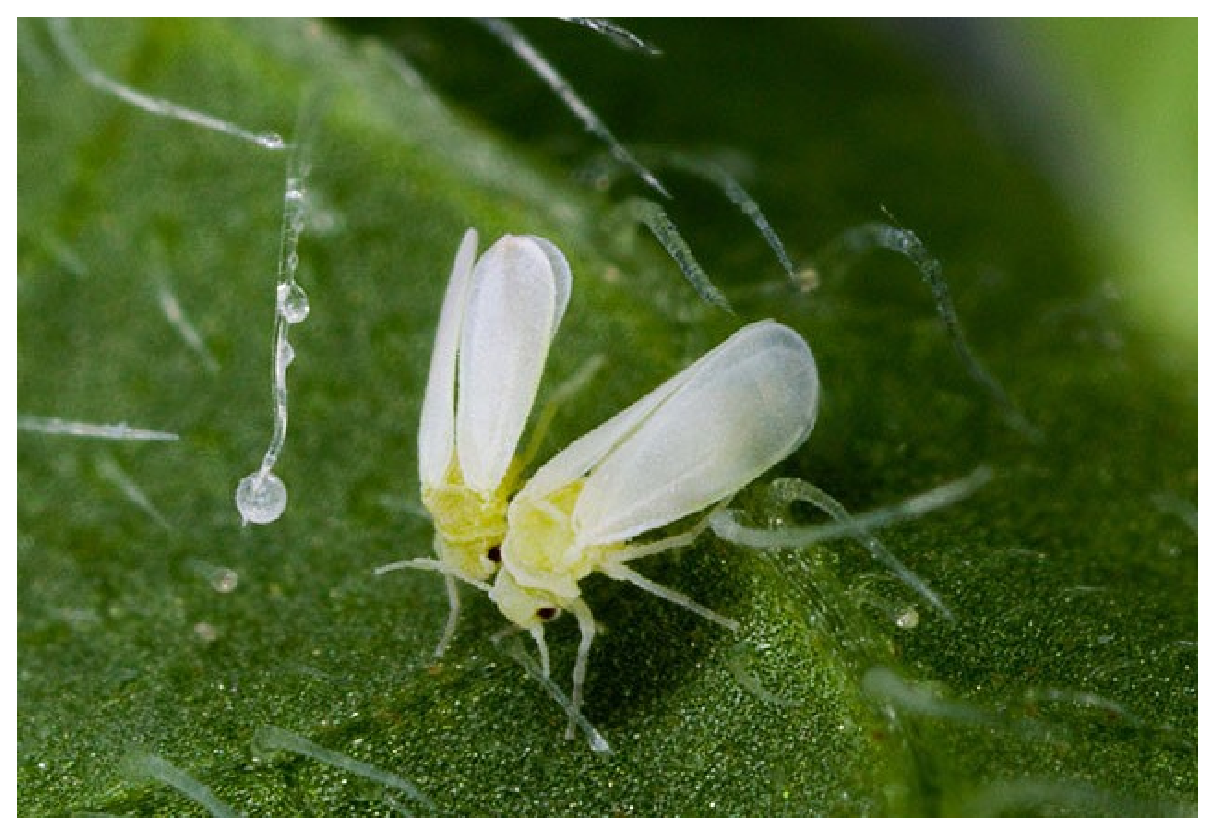
\includegraphics[width=\linewidth]{Feathergraphics/Mosca_Blanca.eps}
\end{textblock*}
\end{frame}

\begin{frame}	
	\begin{textblock*}{60mm}(5mm,20mm)
			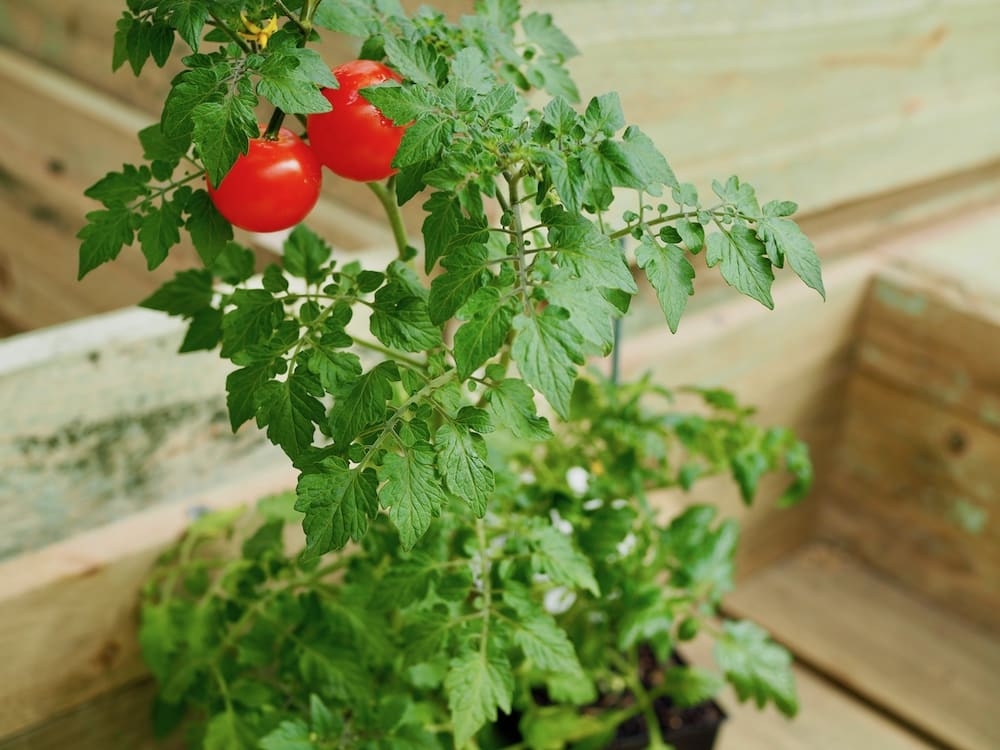
\includegraphics[width=\linewidth]{Feathergraphics/Tomato_plant.eps}
\end{textblock*}
\begin{textblock*}{40mm}(80mm,20mm)
			\includegraphics[width=\linewidth]{Feathergraphics/TYLCV_3_bush.eps}
\end{textblock*}	
\end{frame}

\begin{frame}
\begin{textblock*}{40mm}(10mm,25mm)
			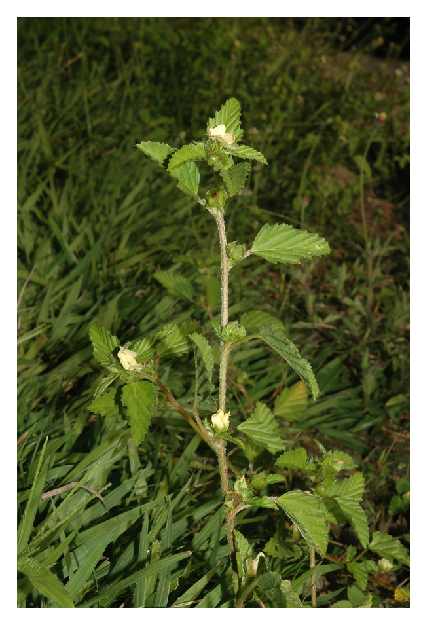
\includegraphics[width=\linewidth]{Feathergraphics/Malvastrum_coromancalianum_L.eps}
\end{textblock*}
\begin{textblock*}{60mm}(60mm,25mm)
			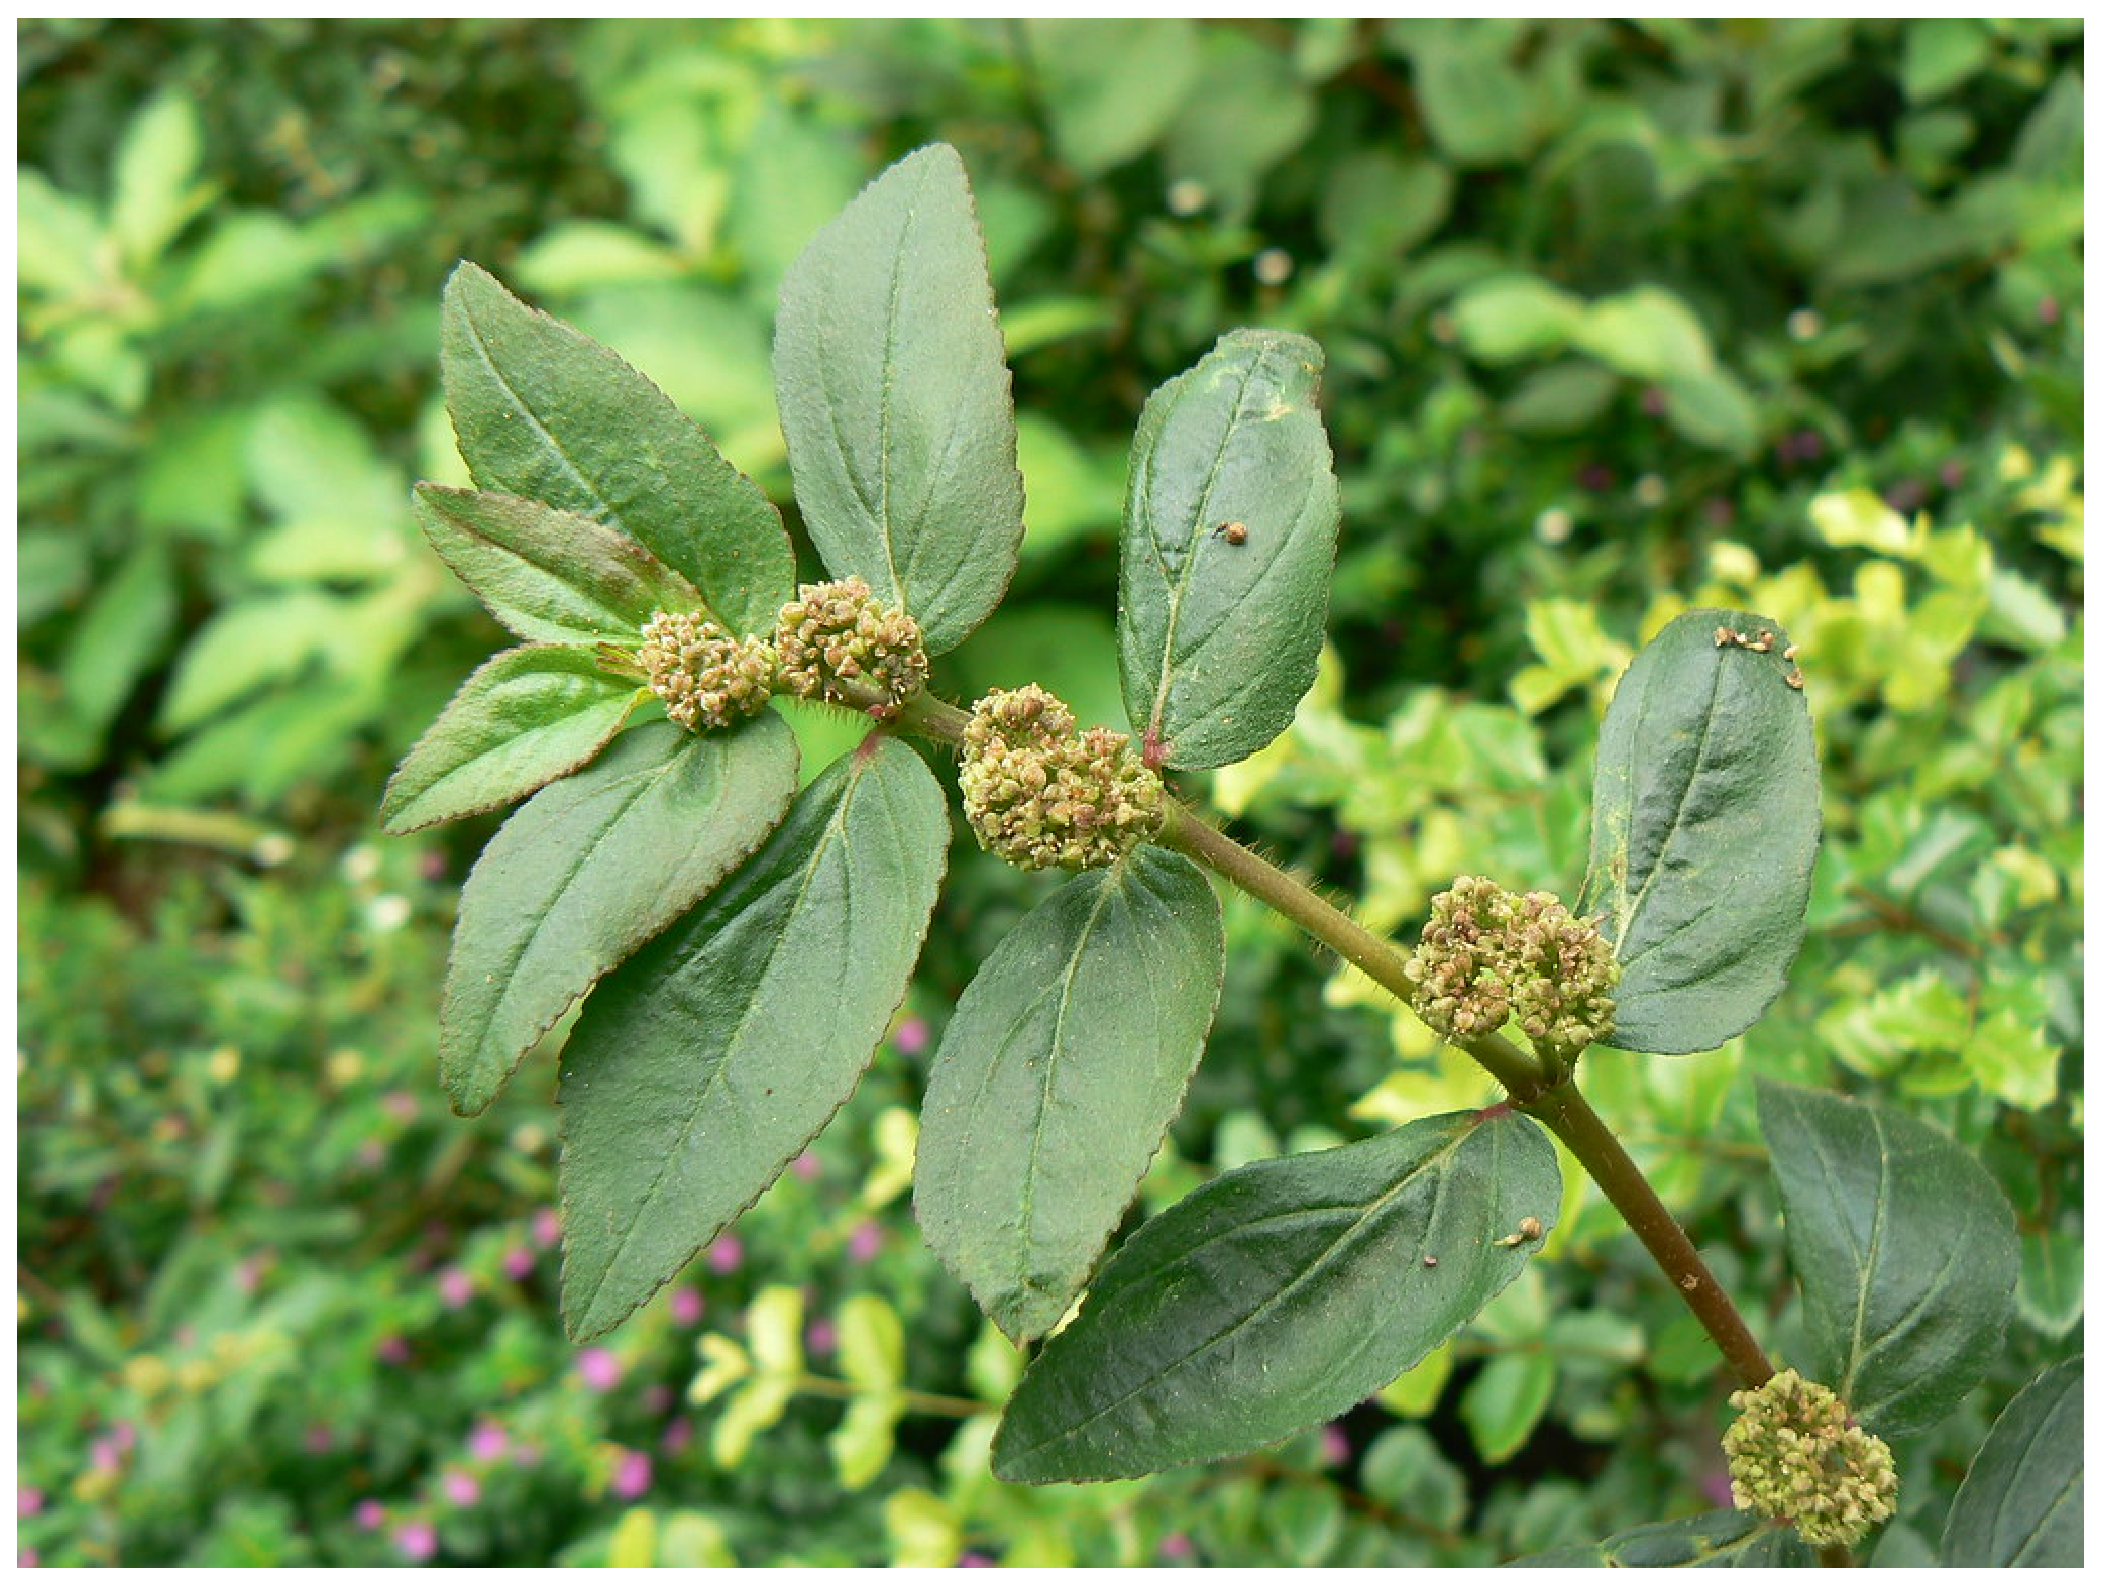
\includegraphics[width=\linewidth]{Feathergraphics/Euphorbia_geniculata_Ort.eps}
\end{textblock*}	
\end{frame}

\section{Objetive}
\begin{frame}{}{}
	\begin{block}{Objetive}
		Model optimal phytosanitary policies for diseases in agricultural crops.
	\end{block}
	
\end{frame}

\section{Epidemical Model}

%%%%%%%%%%%%%%%%%%%%%%%%%%%%%%%%%%%%%%%%%%%%%%%%%%%%%%%%%%%%%%%%%%%%
\begin{frame}{}
\begin{bibunit}[abbrv]
	\nocite{Holt1999b}
	\putbib
\end{bibunit}
\end{frame}

%%%%%%%%%%%%%%%%%%%%%%%%%%%%%%%%%%%%%%%%%%%%%%%%%%%%%%%%%%%%%%%%%%%%%
\begin{frame}{Plant Model without control}{Tomato Leaf Curl Virus Disease Using an Epidemiological Model}
\begin{textblock*}{60mm}(65mm,25mm)
    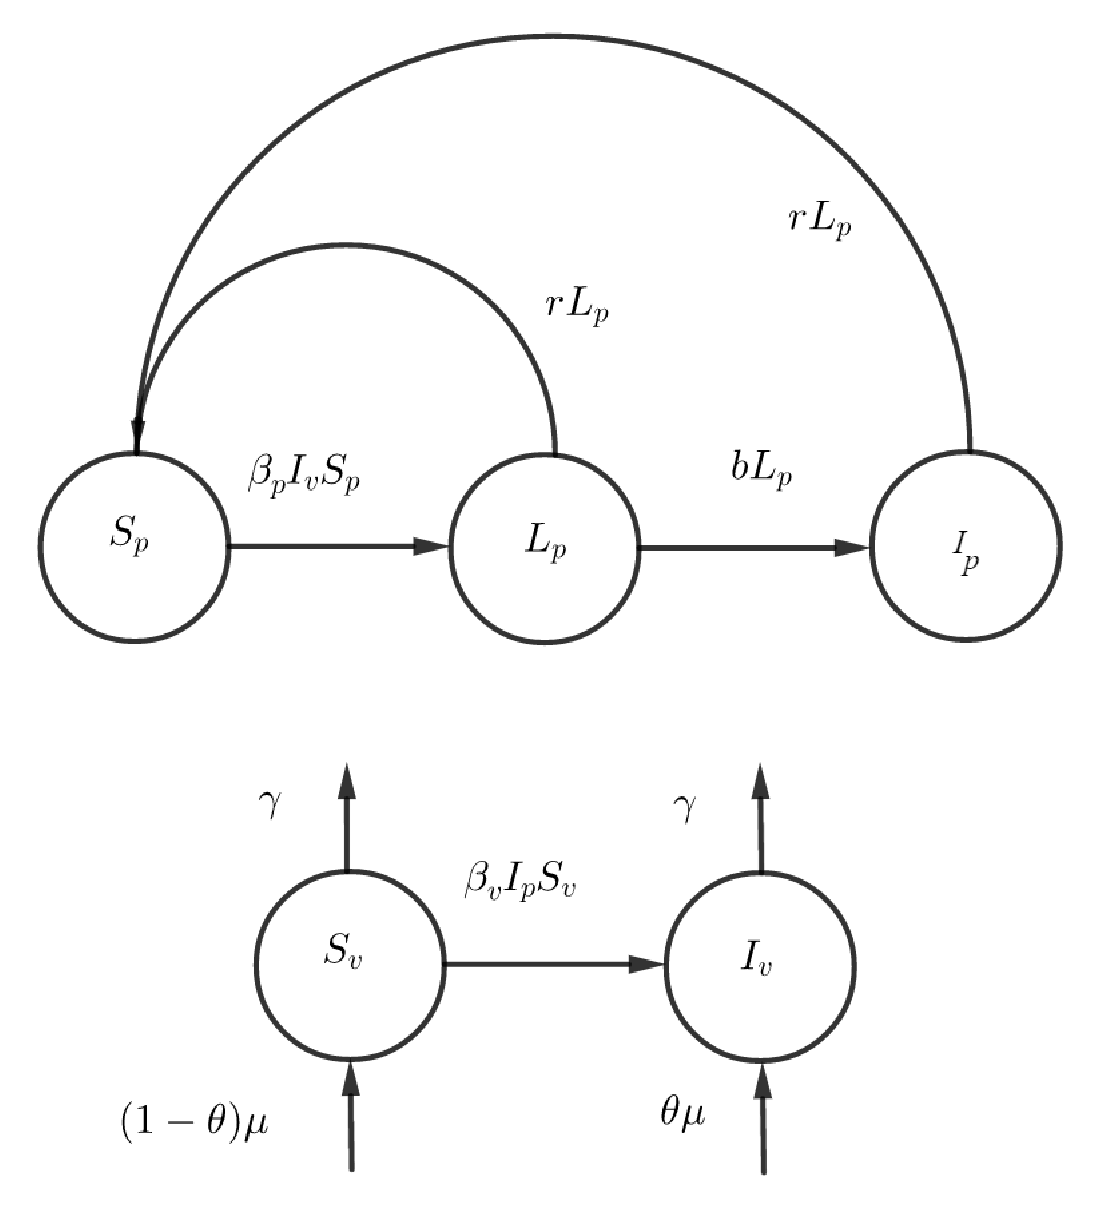
\includegraphics[width=\linewidth]{Feathergraphics/plant_diagram.eps}
\end{textblock*}
\begin{textblock*}{60mm}(5mm,25mm)
	\begin{graybox}{Hypothesis:}
		
		\begin{itemize}
			\item Susceptible plants will become infected when an infected whitefly feeds on it, both latent and infected we will remove and re-plant susceptible plants
			\item Whiteflies become infected when they feed on an infected plant,
			\item there will be entry of whiteflies that come from alternative hosts.
		\end{itemize}
		\end{graybox}	
\end{textblock*}
\end{frame}

\begin{frame}
\frametitle{Others Controls}
\begin{itemize}
	\item Cultural Control.
	\item Physical barriers.
	\item Planting dates.
	\item Removal of infested plants.
	\item Host plant resistance.
	\item Biological control.
\end{itemize}
\end{frame}

\begin{frame}	
		\begin{textblock*}{62mm}(2mm,10mm)
			\begin{greenbox}{Consider the following ordinary differential equations:}
				\begin{align*}
            		\frac{dS_p}{dt} &=-\beta_p S_p I_v +\textcolor{capri}{r}
             			(L_p +  I_p),\\
            		\frac{dL_p}{dt} &= \beta_p S_p I_v -b L_p 
            			-\textcolor{capri}{r} L_p,\\
            		\frac{dI_p}{dt} &= b L_p - \textcolor{capri}{r} I_p,\\
           			\frac{dS_v}{dt} &=-\beta_v S_v I_p - \textcolor{cadmiumorange}{\gamma} S_v   -(1-\theta)\mu,\\
            		\frac{dI_v}{dt} &=  \beta_v S_v I_p -\textcolor{cadmiumorange}{\gamma} I_v	-\theta\mu,\\
								S_p(0) &= S_p_0, L_p(0) = L_p_0, I_p(0) = I_p_0,\\
								S_v(0) &= S_v_0, I_v(0) = I_v_0.
				\end{align*}
			\end{greenbox}
		\end{textblock*}
	
	\begin{textblock*}{60mm}(65mm,10mm)
		\begin{tabular}{|c |c |l |} 
				\hline
				Par. & Value & Descrip. \\ [0.5ex] 
				\hline
				$\beta_p$ & 0.1 & plant latent rate  \\ 
				\hline
				$r$ & 0.01 & plant remove rate \\
				\hline
				$b$ & 0.075 & plant infectious rate\\
				\hline
				$\gamma$ & 0.06 &  vector die or depar rate \\
				\hline
				$\mu$ & 0.3 & immigration rate \\
				\hline
				$\theta$ & 0.2 & infected vectors arrival \\
				\hline
				$\beta_v$ &0.003 & vector infected rate\\ 
				\hline
	\end{tabular}
	\end{textblock*}

	\begin{textblock*}{50mm}(70mm,50mm)
    	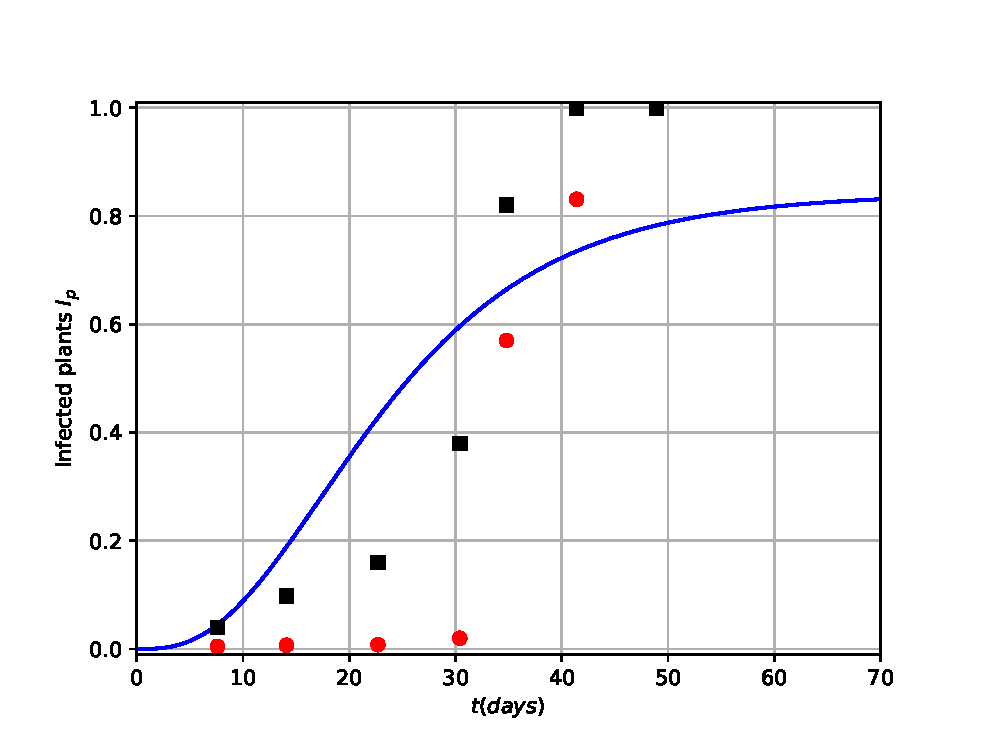
\includegraphics[width=\linewidth]{Feathergraphics/Simulation_data.eps}
	\end{textblock*}
\end{frame}
%-------------------------------------------------------------------------------
\begin{frame}
	\begin{textblock*}{50mm}(5mm,15mm)
		\begin{greenbox}{}
			Computing the $R_0$ we have,
			\begin{equation*}
				R_0=\sqrt{\frac{\beta_v\mu b\beta_p}{r^2(r+b)\gamma}}.
			\end{equation*}
		\end{greenbox}
		
	\end{textblock*}
	\begin{textblock*}{50mm}(70mm,15mm)
		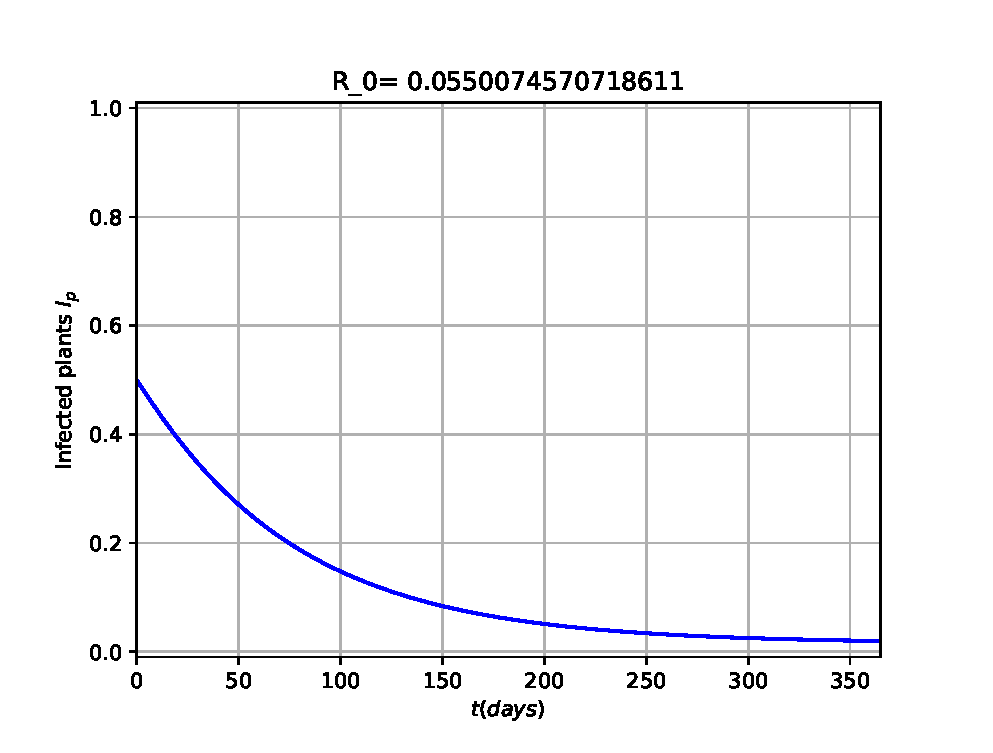
\includegraphics[width=\linewidth]{Feathergraphics/Tomato_simulation_1.eps}
		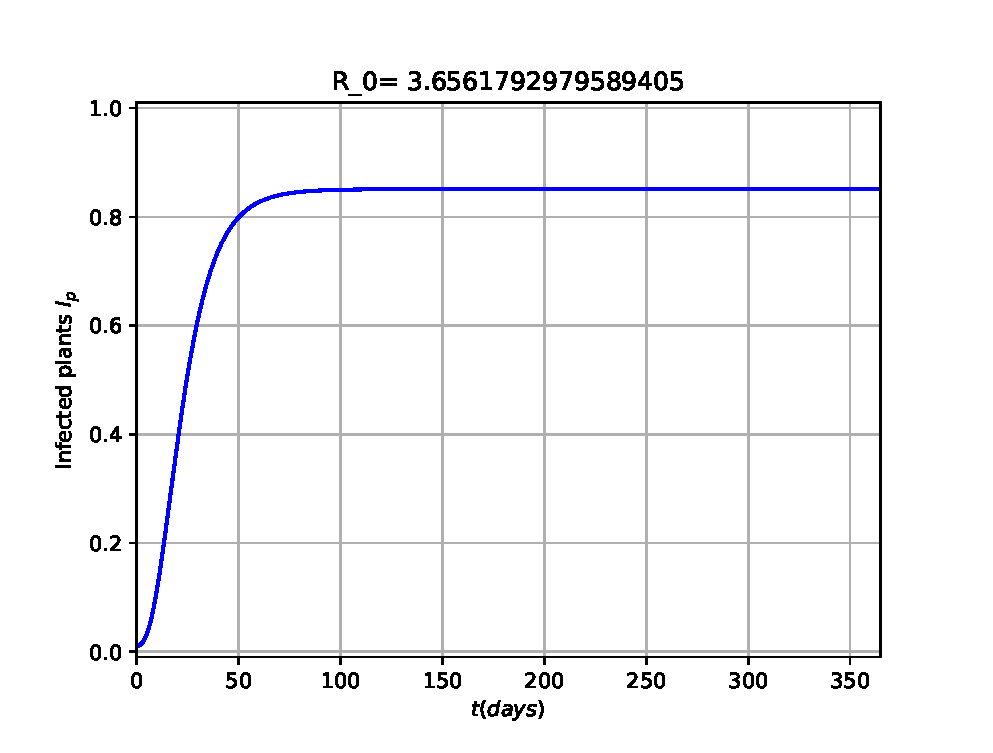
\includegraphics[width=\linewidth]{Feathergraphics/Tomato_simulation_2.eps}
	\end{textblock*}	
\end{frame}
%%-------------------------------------------------------
%%-------------------------------------------------------
%
%%-------------------------------------------------------
%-------------------------------------------------------
\section{Controlled Model}
\subsection{Plant model}
\begin{frame}{Plant Model with control}{Tomato Leaf Curl Virus Disease Using an Epidemiological Model}
The controlled system is the following:

    \begin{equation*}
        \begin{align*}
            \frac{dS_p}{dt} &=-\beta_p S_p I_v +(r +u_1)L_p + (r + u_2) I_p,\\
            \frac{dL_p}{dt} &=\beta_p S_p I_v -b L_p -(r + u_1)L_p,\\
            \frac{dI_p}{dt} &= b L_p - (r + u_2) I_p,\\
            \frac{dS_v}{dt} &=-\beta_v S_v I_p - (\gamma+u_3) S_v -(1-\theta)\mu,\\
            \frac{dI_v}{dt} &=\beta_v S_v I_p -(\gamma+u_3) I_v -\theta\mu,				
        \end{align*}
    \end{equation*}
\end{frame}

\begin{frame}
	With the cost functional:
	\begin{equation*}
	\int_{0}^T
	\left[
	A_1 I_p(t) + A_2 L_p(t) + A_3 I_v(t)
	+ c_1 u_1(t)^2 + c_2 u_2(t)^2 + c_3 u_3(t)^2
	\right] dt.
	\end{equation*}
		
\end{frame}

\begin{frame}
\frametitle{Case with one controls}
\begin{figure}
	\centering	
	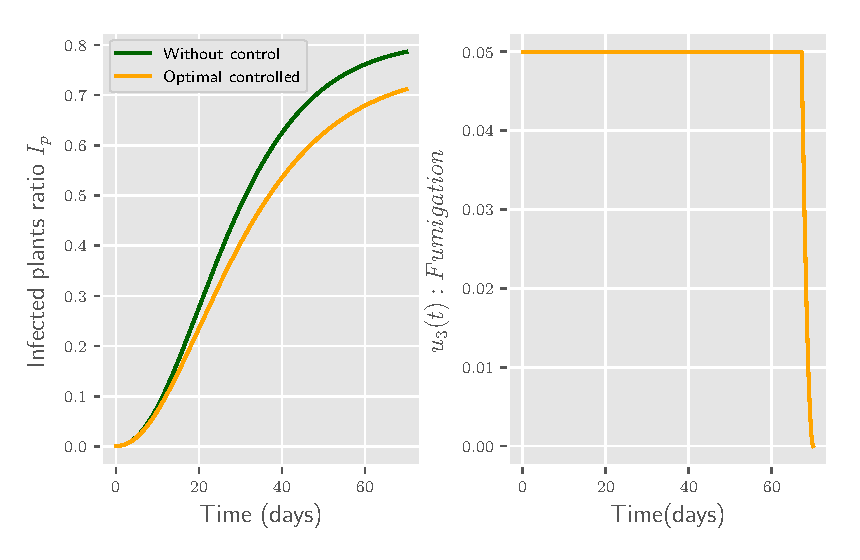
\includegraphics[scale=0.5]{Feathergraphics/figure_1_tomato_one_control.eps}
\end{figure}	
\end{frame}

\begin{frame}
\frametitle{Case with two controls}
\begin{figure}
	\centering	
	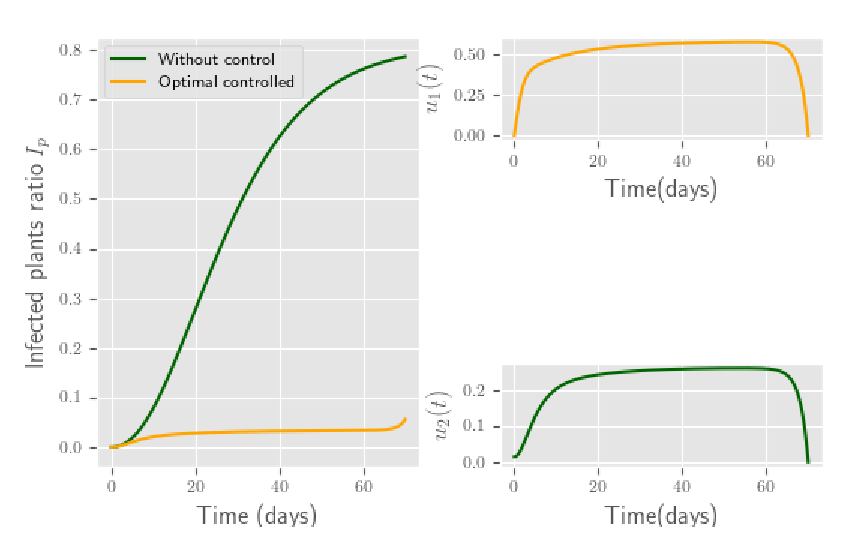
\includegraphics[scale=0.5]{Feathergraphics/two_control_simulation_2.eps}
\end{figure}	
\end{frame}

\begin{frame}
\begin{figure}
\frametitle{Case with three controls}
	\centering	
	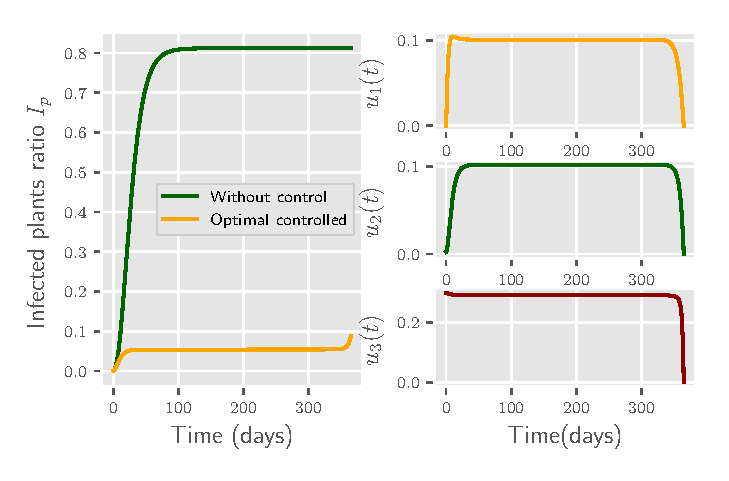
\includegraphics[scale=0.5]{Feathergraphics/three_controls_simulation_1.eps}
\end{figure}	
\end{frame}
%-------------------------------------------------------
%-------------------------------------------------------
%
%% Aquí va la teoria de exitencia y pontryagain
%
%-------------------------------------------------------
%-------------------------------------------------------
\begin{frame}

\begin{textblock*}{65mm}(3mm,10mm)
	\begin{greenbox}{}
		Let $T\in (0,\infty)$ be fixed. Consider the control system:

		$$\left\{ \begin{array}{l}
		\dot{X}(s)=f(s,u(s),X(s))\,\,s\in [t,T], \\
		X(t)=x,\\
		\end{array}
		\right.$$

		with terminal state constraint
		$$X(T;t,x,u(\cdot))\in M,$$
		where $M\subseteq \mathbb{R}^n$ is fixed.
	\end{greenbox}
\end{textblock*}

\begin{textblock*}{55mm}(70mm,10mm)
	\begin{yellowbox}{}
		Any map $M:\mathbb{R}_{+}\rightarrow 2^{\mathbb{R}^n}$ is called a moving target in $\mathbb{R}^n$ if for any $t\in \mathbb{R}_{+}$, $M(t)$ is a measurable set in $			\mathbb{R}^n$.
	\end{yellowbox}
\end{textblock*}
\begin{textblock*}{100mm}(10mm,70mm)
	\begin{yellowbox}{}
		
	\end{yellowbox}
\end{textblock*}
\end{frame}


\begin{frame}

\begin{textblock*}{110mm}(10mm,10mm)
	\begin{graybox}{Problem (C)}
		Let $M(\cdot)$ be a moving target set in $\mathbb{R}^n$. For given $(t,x)\in \mathbb{R}_{+}\times \mathbb{R}^n$, find a control $u(\cdot)\in \mathcal{U}[		t,	\infty)$ 		such that for some $\tau \geq t$,

		$$X(\tau;t,x,u(\cdot))\in M(\tau).$$
	\end{graybox}
\end{textblock*}

\end{frame}

\begin{frame}
\begin{textblock*}{120mm}(5mm,10mm)
	\begin{graybox}{(C1)}
		The map $f:\mathbb{R}_{+}\times U\times \mathbb{R}^n\rightarrow \mathbb{R}^n$ is measurable and there exists a constant $L>0$ such that
				$$\left\{ \begin{array}{l}
				|f(t,u,x_1)-f(t,u,x_2)|\leq L|x_1-x_2|,\, (t,u)\in \mathbb{R}_{+}\times U,\, x_1,x_2\in \mathbb{R}^n,\\
				|f(t,u,0)|\leq L,\,\mbox{for every}\,(t,u)\in \mathbb{R}_{+}\times U .\\
				\end{array}
				\right.$$
	\end{graybox}
\end{textblock*}

\begin{textblock*}{120mm}(5mm,43mm)
	\begin{graybox}{(C2)}
		The maps $g:\mathbb{R}_{+}\times U\times \mathbb{R}^n\rightarrow \mathbb{R}$ and $h.\mathbb{R}^n\rightarrow \mathbb{R}$ are measurable and there exists a continuous function $\omega:\mathbb{R}_{+}\times\mathbb{R}_{+}\rightarrow \mathbb{R}_{+}$, called a local modulus of continuity, which is increasing in each argument, and $\omega(r,0)=0$ for every $r\geq 0$, such that 
$$|g(s,u,x_1)-g(s,u,x_2)|+|h(x_1)-h(x_2)|\leq \omega(|x_1|\vee |x_2|,|x_1-x_2|)$$
$\mbox{for every}\, (s,u)\in \mathbb{R}_{+}\times U,x_1,x_2\in \mathbb{R}^n,$ where $|x_1|\vee |x_2|=\max\{|x_1|,|x_2|\}$.
	\end{graybox}
\end{textblock*}
\end{frame}

\begin{frame}
\begin{textblock*}{120mm}(5mm,10mm)
	For any $(t,x)\in [0,T]\times\mathbb{R}^n$, let us introduce the following set:
	$$\mathbb{E}(t,x)=\{(z^0,z)\in \mathbb{R}\times \mathbb{R}_{+}|z^0\geq g(t,u,x),z=f(t,u,x),\, u\in U\}.$$
	The following assumption gives some compatibility between the control system and the cost functional.
\end{textblock*}

\begin{textblock*}{120mm}(5mm,35mm)
	\begin{graybox}{(C3)}
		For almost all $t\in [0,T]$, the following Cesari property holds for any $x\in \mathbb{R}^n$,

		$$\bigcap_{\delta>0}\bar{co}\mathbb{E}(t,B_{\delta}(x))=\mathbb{E}(t,x),$$

		where, we recall that $B_{\delta}(x)$ is the open ball centered at $x$ with radius $\delta>0$, and $\bar{co}(E)$ stands for the closed convex hull of the set $E$ (the 	smallest closed convex set containing E).
	\end{graybox}
\end{textblock*}


\end{frame}







\begin{frame}
	\begin{textblock*}{120mm}(5mm,15mm)
		\begin{graybox}{Existence Theorem}
			Let (C1)-(C3) hold. Let $M\subseteq \mathbb{R}^n$ be a non-empty closed set. Let $(t,x)\in [0,T]\times\mathbb{R}^n$ be given and $\tilde{\mathcal{U}}^M_x[t,T]\neq\emptyset$. Then problem $(OC)^T$ admits at least one optimal pair.
		\end{graybox}
	\end{textblock*}
\end{frame}
%-------------------------------------------------------
%   Pontryagain
%-------------------------------------------------------

\begin{frame}

\end{frame}


\end{document}